\documentclass[amsmath,amssymb,amsfonts,aps,pre,preprint,superscriptaddress,showpacs,showkeys,longbibliography,nofootinbib]{revtex4-1}
%\documentclass[12pt]{article}
%\documentclass[jcp,aps,final,preprint,groupedaddress,showpacs,
%floatfix,aip,reprint,amssymb,lengthcheck]{revtex4-1}
%\documentclass[jcp,preprint,final,aip,groupedaddress,floatfix,amssymb,lengthcheck]{revtex4-1}
\hyphenation{Keeping Thoroughly}

\usepackage{caption}
\usepackage{mathtools}
\usepackage{epsfig}
\usepackage[english]{babel}
\usepackage{color}
\usepackage{subcaption}
\usepackage{hyperref}
\usepackage{lipsum}
\usepackage{xcolor}
\usepackage{amsthm}
\usepackage{physics}
\usepackage{float}

\newcommand{\sgn}{\operatorname{sgn}}
\newcommand{\err}{\operatorname{Err}}
\newcommand*{\logten}{\mathop{\log_{10}}}
\newcommand*{\lop}{\mathcal{L}\,}
\newcommand*{\nlop}{\mathcal{N}\,}
\newcommand*{\rop}{\mathcal{R}\,}
% \DeclareMathOperator\erf{erf}
\newcommand{\Var}{\mathrm{Var}}

\AtBeginDocument{%
    \newwrite\bibnotes
    \def\bibnotesext{Notes.bib}
    \immediate\openout\bibnotes=\jobname\bibnotesext
    \immediate\write\bibnotes{@CONTROL{REVTEX41Control}}
    \immediate\write\bibnotes{@CONTROL{%
    apsrev41Control,author="08",editor="1",pages="1",title="0",year="1"}}
     \if@filesw
     \immediate\write\@auxout{\string\citation{apsrev41Control}}%
    \fi
}%

\newtheorem{thm}{Theorem}

\newcommand{\me}{\mathrm{e}}
\newcommand{\pa}{\partial}
\DeclareMathOperator{\erfc}{erfc}

\begin{document}
\title{An analytic moving-junction approximant to the traveling wave solution of the classical Fisher-KPP equation}

\author{Orjan Ameye}
\affiliation{Institute for  Theoretical Physics, KU Leuven, B-3001 Leuven, Belgium}

\author{Jonas Berx}
\affiliation{Institute for  Theoretical Physics, KU Leuven, B-3001 Leuven, Belgium}

\author{Joseph O. Indekeu}
\affiliation{Institute for  Theoretical Physics, KU Leuven, B-3001 Leuven, Belgium}

\date{\today}

\begin{abstract}
An analytic approximation is devised which captures both long-time asymptotic as well as transient features of the traveling-wave solution to the classic nonlinear Fisher-KPP equation for diffusion and growth of a population. The approximant consists of a moving junction between an advancing front and a nearly-saturated domain, obtained by matching two linearized versions of Fisher-KPP equation. The long-time asymptotic behavior of the front velocity is coincident with that of the critical case between pushed and pulled fronts, within the saturation-at-a-moving-boundary reduction of Fisher-KPP studied by Berestycki {\em et al}. The transient feature concerns the diffusion-driven depletion and subsequent recovery of the population on the saturated side of the moving junction. A quantitative  improvement of the analytical approximant is obtained by applying the BLUES function method to the nonlinear Fisher-KPP equation. 
\end{abstract}

\maketitle

\section{Introduction}\label{sec:intro}
Differential equations (DEs) are one of the most powerful mathematical tools in describing problems in exact sciences. For solving fairly complicated DEs, e.g., nonlinear equations, one often seeks recourse to numerical methods. Numerical solutions are usually helpful in probing the results of the model, yet they provide little insight in how these results came to be and in the physical structure that lies behind them. Therefore, it is often useful to employ analytical approximation techniques to find an approximant to the solution. Perturbation theory, the Adomian decomposition method (ADM) and various schemes based on the variational iteration method (VIM) are common choices in this regard. In this work, we make use of another approach, which is the reduction of a nonlinear DE to a linear DE supplemented with a set of constraints. This starting point bears similarity to the one studied in  \citet{Berestycki2017}. Next, we explore an analytic refinement by means of the recently developed Beyond-Linear-Use-of-Equation-Superposition method (BLUES) for nonlinear DEs \cite{Indekeu_2018,Berx_2020,Berx_2021}.

In this work, the nonlinear partial differential equation (PDE) of interest is the Fisher–\\Kolmogorov–Petrovsky–Piskunov equation (Fisher-KPP equation for short) \cite{fisher1937wave, kolmogorov1937study}, a reaction-diffusion equation which has been useful in the physical characterization of many natural systems \cite{canosa1973nonlinear,ross2010generalized,hamel2011speedup, Bewick2017Invasion, Demaerel_2019}, e.g., in modeling the growth and diffusion of biological systems or physical active matter \cite{fisher1937wave}. A particular class of solutions of this PDE are traveling waves or wavefronts. These solutions are characterized by a fixed shape and a constant propagation velocity. The search for wavefront solutions of the Fisher-KPP equation and generalizations thereof has a long history and has enjoyed renewed activity in recent years \cite{Mishra2012,Mansour2010,Yuan2013general}.  It has long been proven that under initial conditions with compact support the solution of the Fisher-KPP equation evolves to a traveling wave solution with a constant velocity \cite{kolmogorov1937study, bramson1983,Roberts13}. Yet, no exact solutions have been obtained except for a special value of the propagation velocity \cite{Ablowitz1979}. For a thorough review of this exciting field we refer the reader to \cite{VANSAARLOOS200329}.

Our goal is twofold. We aim at constructing in (piece-wise) analytic form the simplest possible but non-trivial time- and space-dependent emergent traveling wave approximant that qualitatively respects the boundary conditions as well as the asymptotic (long-time) behavior of the solution to the Fisher-KPP equation. Subsequently, we explore to what extent a systematic refinement of this approximant is feasible, while maintaining simplicity and closed-form analytic expressions. 

In order to satisfy the boundary conditions at, respectively, $x\to\pm\infty$, two distinct linear PDEs are defined, which capture the saturation of the solution in the vicinity of the carrying capacity and the decay of the solution to zero at the foot of the advancing front. The initial condition is chosen to be the Heaviside step function, centered about $x=0$, which respects both boundary conditions. The solutions of the two PDEs are subsequently matched at their common point of intersection (the junction). This provides a piecewise analytic approximant which evolves towards a traveling wavefront, which features a singularity (jump in slope) at the junction. This combined profile is a simple weakly-singular approximation that displays the features of the emergent traveling wave correctly. In particular, it fulfills the boundary conditions and develops a fixed shape which selects the correct constant universal ``pulled-front" velocity for long times. In addition, for short times, the diffusion-driven depletion and subsequent recovery of the concentration on the saturated side of the moving junction is qualitatively respected by the approximant.

In the second step we test available calculational approaches on their suitability for providing an improvement over the approximant obtained by matching two linear problems, by going beyond the linear domain. Among three different methods, ADM, VIM and BLUES, the latter is the one with the help of which we can obtain a quantitative improvement. The approximant  resulting in the first iteration, which includes an effect of the nonlinear growth term in the DE, is given analytically in compact closed form.  

This paper is structured as follows. First, in Section \ref{sec:constructing_approximant} the construction of the piecewise-analytic approximant for the emergent traveling wave solution of the Fisher-KPP equation is presented. Next, in Section \ref{sec:properties}, physical properties are computed and compared with those of the numerical solution. With the help of the BLUES method a refinement of the approximant is calculated in section \ref{sec:refinement}. Finally, in Section \ref{sec:conclusion}, a conclusion is presented.

\section{Construction of the wavefront approximant}\label{sec:constructing_approximant}

To set the stage, we consider the classical Fisher-KPP equation
\begin{align}\label{eq:dimensionfull_Fisher}
    u_t - Du_{xx} - \alpha u(1-u)=0,
\end{align}
defined on $(x,t) \in \mathbb{R} \times [0,\infty)$ with $u_t\equiv\partial u / \partial t$,  $u_{xx}\equiv\partial^2 u / \partial x^2$.  In general, it describes the growth of a (dimensionless) density or population fraction $u(x,t)$ subject to diffusion. In this work it suffices to take $u(x,t)\in[0,1]$ in which the lower bound and higher bound represent the extinction and the carrying capacity, respectively. The growth rate $\alpha$ and the diffusion constant $D$ can be scaled out by considering the transformations $t\gets \alpha t$ and $x\gets \sqrt{\alpha/D}\,x$, which render both $x$ and $t$ dimensionless. This results in the dimensionless PDE
\begin{align}\label{eq:dimensionless_Fisher}
    \nlop u(x,t)\equiv u_t - u_{xx} - u(1-u)=0.
\end{align}
where $\mathcal{N}$ is a nonlinear differential operator acting on the solution $u(x,t)$.

To construct an approximant for the emergent traveling wave solution of the Fisher-KPP equation one must first ask the question for which initial condition $f(x)$ one can obtain such a solution. Actually, since Ref. \cite{bramson1983}, it is known that when $f(x)\in[0,1]$, $f(-\infty)=1$, $f(\infty)=0$ and $f$ has compact support, i.e.,
\begin{align}\label{eq:compact support}
\int \dd{x} f(x) x e^{x}<\infty,
\end{align}
then the solution $u(x, t)$ of the Fisher-KPP equation \eqref{eq:dimensionless_Fisher} evolves towards a traveling wave solution, $u(x, t) \to \omega(x - v^* t)$, of a non-trivial shape $\omega$ with a (dimensionless) propagation speed $v^*=2$ (``pulled front" case). Furthermore, if one defines a co-moving coordinate $\mu_t$ as $u(\mu_t, t)=a$ with $a\in(0,1)$, it is known that
\begin{align}
\label{generic}
    \mu_{t}=2 t-\frac{3}{2} \ln t+C+o(1) \quad \text { as } t \rightarrow \infty,
\end{align}
with $C$ a constant depending on $a$. In this context the most obvious initial condition is the Heaviside step function 
\begin{equation}
    \label{eq:initial_condition}
    u(x,0)=f(x)=\Theta(-x).
\end{equation}

An emergent traveling wave solution has a couple of central features which an approximant favorably possesses. It must respect the spatial boundary conditions. In the case of the Fisher-KPP equation with initial condition \eqref{eq:initial_condition} these will be $\lim_{x\rightarrow-\infty}u(x, t)=1$ and $\lim_{x\rightarrow\infty}u(x, t)=0$. The shape of the wavefront must asymptotically become stationary. And, by virtue of the previous property, one can define a unique propagation velocity $v^*$ for the wavefront.

The strategy of finding the approximant goes as follows. The behavior of the solution $u(x,t)$ near the uniform steady states $u=0$ and $u=1$ can be captured by two related linear PDEs
\begin{align}
\label{eq:linear_operator_Right}
    \mathcal{L}_R \, u &= \partial_t u -\partial_{xx}u - u=0,\\
    \mathcal{L}_L \,  u &=\partial_t u -\partial_{xx}u - (1-u)=0.
    \label{eq:linear_operator_Left}
\end{align}
Let us name them the ``right" and ``left" linear PDE as they will, respectively, and asymptotically in space, describe the right and left part of the exact solution of the Fisher-KPP equation \eqref{eq:dimensionless_Fisher} with Heaviside initial condition. It is natural to involve both of these linear PDEs because together they guarantee the spatial boundary conditions for a traveling wave. The approximate solution to the nonlinear PDE can then be obtained using a matching procedure in which the right and left trial solutions are combined.

For later convenience (anticipating an iteration procedure), we can rewrite the PDEs in an inhomogeneous form by invoking the initial condition $f(x)$ through the action of a Dirac-delta source in time, which yields
\begin{align}
\label{eq:linear_operator_Right_Alt}
    \mathcal{L}_R \, u &= \partial_t u -\partial_{xx}u - u=f(x)\delta(t),\\
    \mathcal{L}_L \,  u &=\partial_t u -\partial_{xx}u - (1-u)=f(x)\delta(t),
    \label{eq:linear_operator_Left_Alt}
\end{align}
where it is understood that $u(x,t)=0$ for $t<0$. Above equivalence holds if $\mathcal{L}$ contains a first (but no higher) derivative with respect to time $t$ \cite{Berx_2021}, which is the case for the Fisher-KPP equation \eqref{eq:dimensionless_Fisher}. These inhomogeneous linear PDEs are solved by
\begin{align}
 \label{eq:rewriten_linear_operator_delta_u}
	\lop u(x, t)=\lop \int_{0^{-}}^{t} \dd{s} \int_{\mathbb{R}} \dd{y} G\left(x-y, t-s\right) f\left(y\right) \delta\left(s\right)=f(x) \delta(t),
\end{align}
which is a two-variable convolution $u(x, t) = G \ast f \delta$ of the corresponding Green function and initial condition ``source''. The Green functions of these linear problems are obtained by solving  $\lop G(x,t)=0$ with $\lim_{t\to 0}G(x,t)=\delta(x)$. 

% Notice that the right linear problem has a constant term in its expression, this will yield a constant term in the Green function which would give in infinities in the convolution. Hence, the problem for the left linear PDE must be rewritten to
% \begin{align}\label{eq:modified_nonlinear_operator_Left}
%     \mathcal{N}^*\, u &=\mathcal{N}\, u+1= \pa_t u -\pa_{xx}u - u(1-u)+1=1+f(x)\delta(t),\\
%     \mathcal{L}^*_L \, u &=\pa_t u -\pa_{xx}u +u=1+f(x)\delta(t),
%     \label{eq:modified_linear_operator_Left}
% \end{align}
% which is equivalent to the original description \eqref{eq:linear_operator_Left}. 

% The Green functions of these linear problems are obtained by solving 
% $\lop G(x,t)=0$ with $\lim_{t\to 0}G(x,t)=\delta(x)$ and are given by
% \begin{align}
%     G_R(x,t) = e^{t}\frac{e^{\frac{x^2}{4 t}}}{\sqrt{4 \pi t}}, \qq{and}
%     G^*_L(x,t) = e^{-t}\frac{e^{\frac{x^2}{4 t}}}{\sqrt{4 \pi t}}.
% \end{align}
\begin{figure}[t]
    \centering
    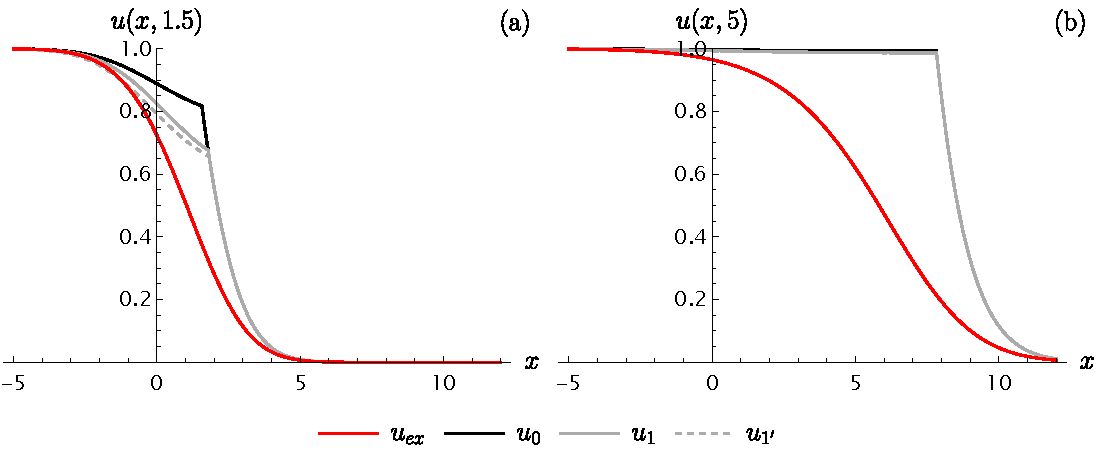
\includegraphics[width=\linewidth]{Figures/PiecewiseApproxGridAlt.pdf}
    \caption{Piecewise analytical construction of $u_0$ \eqref{eq:zeroth_piecewise_approx} (full black line) with moving junction (corner), joining the solutions for ``left" \eqref{eq:linear_operator_Left} and ``right" \eqref{eq:linear_operator_Right} linear PDEs with Heaviside initial condition. The construction of the refined approximant $u_1$ obtained in first iteration using the BLUES function method (full grey line, partly hiding the black line for larger $x$) with moving junction (corner) is also shown. For comparison the  numerically exact solution  of the Fisher-KPP equation is  displayed (smooth full red line). The times of these snaphots are $t=1.5$ in panel (a) and $t=5$ in panel (b). For short times $u_1$ is clearly a better approximation than $u_0$. For $t=5$, at the resolution of the figure, both piecewise analytic approximants $u_0$ (black)  and $u_1$ (grey) have already converged to their common fixed form.}
    \label{fig:PiecewiseApproxAlt2}
\end{figure}

The pertinent solutions of the linear PDEs \eqref{eq:linear_operator_Right} and \eqref{eq:linear_operator_Left} are the following,
\begin{align}\label{eq:BLUES_zero_iteration_Right}
       u^{(0)}_R(x,t)&= \int_{0}^{t} \dd{s}\int_{\mathbb{R}} \dd{y} e^{t-s}\frac{e^{\frac{(x-y)^2}{4 (t-s)}}}{\sqrt{4 \pi (t-s)}} \Theta(-y)\delta(s) 
       = \frac{1}{2} e^t \erfc\left(\frac{x}{2 \sqrt{t}}\right),\\
       u^{(0)}_L(x,t) &= \int_{0}^{t} \dd{s}\int_{\mathbb{R}} \dd{y} e^{-(t-s)}\frac{e^{\frac{(x-y)^2}{4 (t-s)}}}{\sqrt{4 \pi (t-s)}} (\Theta(-y)\delta(s)+1) 
       =  1-\frac{1}{2} e^{-t} \left(1+\text{erf}\left(\frac{x}{2 \sqrt{t}}\right)\right),
       \label{eq:BLUES_zero_iteration_Left}
    \end{align}
where the superscript $0$ indicates that this is a primitive or ``zeroth" approximation and $\erf(.)$ and $\erfc(.)$ are, respectively, the error function and complementary error function. 

It is worthwhile to note here that these simple solutions are non-trivial. One easily verifies that the trivial exponential traveling tail solution $A \exp{-(x-2t)}$ with velocity 2 solves the ``right" linear PDE in \eqref{eq:linear_operator_Right_Alt}. However, it does not satisfy the initial condition, and behaves qualitatively differently from \eqref{eq:BLUES_zero_iteration_Right}. The latter asymptotically features a Gaussian decay instead of an exponential decay, for $(x -2t)\to \infty$.

In Figure \ref{fig:PiecewiseApproxAlt2}, the moving parts of the solutions for the ``right" and ``left" PDE are plotted for different fixed times. For comparison, the numerically exact solution of the Fisher-KPP PDE is drawn in red. One observes that the left and right boundary conditions are satisfied for all profiles. Furthermore, note that the solution of the ``right" PDE $u^{(0)}_R$ meets the solution of the ``left" PDE $u^{(0)}_L$ at an intersection point $x^*_0$, which defines the moving junction. This junction provides the opportunity to construct a piecewise analytic approximant to the exact emergent wavefront solution of the Fisher-KPP equation. The result is conspicuous in Figure \ref{fig:PiecewiseApproxAlt2}. In particular, one can combine the left and right approximants as follows,
\begin{align}\label{eq:zeroth_piecewise_approx}
    u_0(x,t)\equiv
    \begin{cases}
    u^{(0)}_{L}(x,t) \qq{for} x\leq x^*_0(t)\\
    u^{(0)}_{R}(x,t) \qq{for} x>x^*_0(t)
    \end{cases}
    \qq{with} x^*_0(t) = 2\sqrt{t}\erfc^{-1}\left(\frac{2}{1+e^{t}}\right)\,.
\end{align}
The moving junction $x^*_0(t)$ can be seen as a moving boundary between the solutions of the ``left" and ``right" PDEs. Interestingly, asymptotically for $t\to \infty$, the solution of the ``right" linear PDE $u^{(0)}_R$, considered to the right of the moving junction $x^*_0(t)$, converges towards one of the solutions obtained by imposing saturation at a moving boundary as studied in \cite{Berestycki2017}. The solution we have composed does not correspond to the generic ``pulled front" case for which \eqref{generic} holds, but rather resembles that for the ``critical case" between ``pulled" and ``pushed", identified in \cite{Ebert,Berestycki2017}, for which a modified velocity law is valid (see next section). \footnote{For $t\to \infty$, one finds that $u^{(0)}_R(x^*_0, t)\equiv \alpha=1$ and $\partial_x u^{(0)}_R(x^*_0, t)\equiv \beta=-1$ so that the condition $\alpha + \beta = 0$ in \citet{Berestycki2017} is fulfilled.} The reason why we obtain this modified velocity law is simply because we have linearized the DE about the solution for the linearly unstable state \cite{Ebert}. This implies that our approximant runs ahead of the numerical solution.


\section{Properties of the wavefront approximant} \label{sec:properties}
In section \ref{sec:constructing_approximant} we discussed  three necessary properties of an emergent wavefront: it respects the boundary conditions for all times $t\geq0$, its shape remains fixed asymptotically for large $t$ and it then attains a constant velocity. We now show that these requirements are satisfied for the approximant $u_0$.  The first condition is satisfied by construction. To examine the emergent fixed shape and constant velocity, we consider the error $\epsilon(t)$ of the wavefront approximant relative to the numerically exact solution $u_{ex}(x,t)$, defined as the spatial $L^2-$norm
\begin{align}\label{eq:Error}
    \epsilon(t) \equiv ||u_{ex} - u_0||_2^2 =  \int_{\mathbb{R}} \abs{u_{ex}-u_0}^2\dd{x}\,.
\end{align}
\begin{figure}[t]
    \centering
    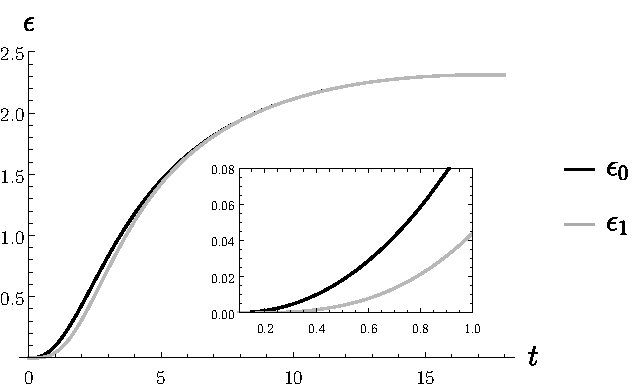
\includegraphics[width=0.7\linewidth]{Figures/Error.pdf}
    \caption{ The $L^2-$norm error $\epsilon (t)$ of the approximants $u_0(x,t)$ ($\epsilon_0$, black line) and $u_1(x,t)$ ($\epsilon_1$, grey line) relative to the numerically exact solution of the Fisher-KPP equation with Heaviside initial condition. The error saturates for long times, consistently with what is seen in panel (b) of Figure \ref{fig:PiecewiseApproxAlt2}. The inset shows detail for short times.}
    \label{fig:error}
\end{figure}
We find (see Figure \ref{fig:error}) that the error saturates to a finite value for long times. This indicates that asymptotically for large $t$, the shape of also $u_0$ remains fixed. 
Let us now verify the propagation velocity of the wavefront approximant $u_0$. From the asymptotic form of the front for long times, i.e., $t\gg1$, it is apparent that the ``right" component $u^{(0)}_{R}$ determines the propagation velocity. Inverting $u^{(0)}_{R}$, as given in \eqref{eq:BLUES_zero_iteration_Right}, with respect to $x$ and taking the limit $t\to\infty$ of the partial derivative with respect to time yields
\begin{align}\label{eq: v* u^0}
  v^*\equiv \left.\lim_{t\to\infty}\partial_t (u^{(0)}_{R})^{-1}(u,t)\right|_{u=const} =2 -\frac{1}{2t} + o\left(\frac{1}{t}\right).
\end{align}
This asymptotic behavior has been verified analytically by using the asymptotic expansion \cite{abramowitz+stegun} for $\erfc(.)$ featured in equation \eqref{eq:BLUES_zero_iteration_Right}. The solution for the ``right" linear PDE, $u^{(0)}_{R}$, uniquely selects the physical velocity of the Fisher-KPP equation \cite{brunet2016}, as would be expected for a ``pulled" front. However, the asymptotic relaxation \eqref{eq: v* u^0}, with leading correction $-1/(2t)$ instead of $-3/(2t)$ corresponds to the ``critical case" in \citet{Berestycki2017}. Note that this is at first sight surprising, but it could have been anticipated in view of the fact that our zeroth approximant features the same standard Green function as that which occurs in the Brownian branching process, for which \eqref{eq: v* u^0} was derived in \cite{brunet2016}.
\begin{figure}[t]
    \centering
    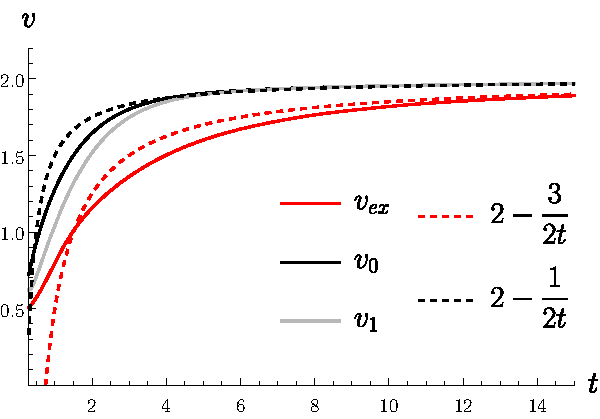
\includegraphics[width=0.6\linewidth]{Figures/Velocity1.pdf}
    \caption{The propagation velocity $v(t)$ of the approximants $u_0(x,t)$ ($v_0$, black line) and $u_1(x,t)$ ($v_1$, grey line) evaluated at the moving junctions $x_0^*(t)$ and $x_1^*(t)$, respectively, and compared with the propagation velocity of the numerically exact solution of the Fisher-KPP equation (red line) evaluated on the moving front with $u_{ex} = 0.5$ fixed. Also shown are the leading asymptotic algebraic corrections in $1/t$ (upper black dashed line $2-1/(2t)$ and lower red dashed line $2-3/(2t)$. }
    \label{fig:Velocity}
\end{figure}

In figure \ref{fig:Velocity} the propagation velocity of the approximant is shown and compared to that of the numerically exact solution. The leading asymptotic behavior for long times is also displayed for each (dashed lines). The generic $1/t$ correction with (universal) prefactor $3/2$ (applicable to "pulled" fronts \cite{VANSAARLOOS200329, brunet2016}) is recovered for the numerically exact solution, whereas the (non-universal) prefactor $1/2$ applies to our approximant, which belongs to the ``critical case" discussed in \cite{Berestycki2017}.

Having confirmed three central features of a traveling wave, we now turn to the calculation of some other physical properties of the piecewise-analytic approximant. For example, one can examine the time evolution of the population $u$ at a fixed position $x>0$, to the right of the position of the step of the initial condition $f(x) = \Theta(-x)$. A characteristic time $\tau$ can be found, needed for the solution $u$ to reach saturation. This can be seen in Fig. \ref{fig:GridSimoide}(a). Naturally, for fixed position $x=\tilde x$, the numerically exact solution exhibits growth of the population from $u=0$ to 1. This function $u(\tilde x,t)$ converges to a fixed sigmoidal shape for $\tilde x\gg 1$. In contrast, the approximant $u_0$ \eqref{eq:zeroth_piecewise_approx} at fixed position converges to a fixed shape consisting of a fast (Gaussian) turn-on on a time scale of the order of unity ($\tau \approx 2$), followed by a plateau at $u_0 =1$. This characteristic time scale can also be estimated using the spatial profile Fig. \ref{fig:PiecewiseApproxAlt2}, panel (b), and taking into account that the velocity of the front is close to $v=2$. Note that the saturation time of the approximant $\tau_0$ is shorter than the saturation time of the numerically exact solution $u_{ex}$. 

One can likewise examine what happens at positions $x<0$ close to $x=0$. The physical phenomenon that takes place here is a competition between growth and diffusion. The diffusion in the vicinity of the sharp drop in the population causes the depletion to travel backwards and drives a depletion of $u$ at $x<0$. This is counteracted by the growth term which acts so as to pull the population back up to its carrying capacity $u=1$. As a result the depletion is transient and the population fully recovers in a short time. The function $u(\tilde x,t)$ exhibits a skewed dip in time, at fixed $\tilde x <0$, as shown in Fig. \ref{fig:GridSimoide}(b). The width of the dip corresponds to a characteristic healing time $\gamma$. The characteristic time of the approximant, $\gamma_0$, is considerably shorter than the characteristic time of the numerically exact solution $\gamma_{ex}$, but the existence and qualitative shape of the diffusion-driven depletion and growth-driven recovery are captured by $u_0$. 
\begin{figure}[t]
    \centering
    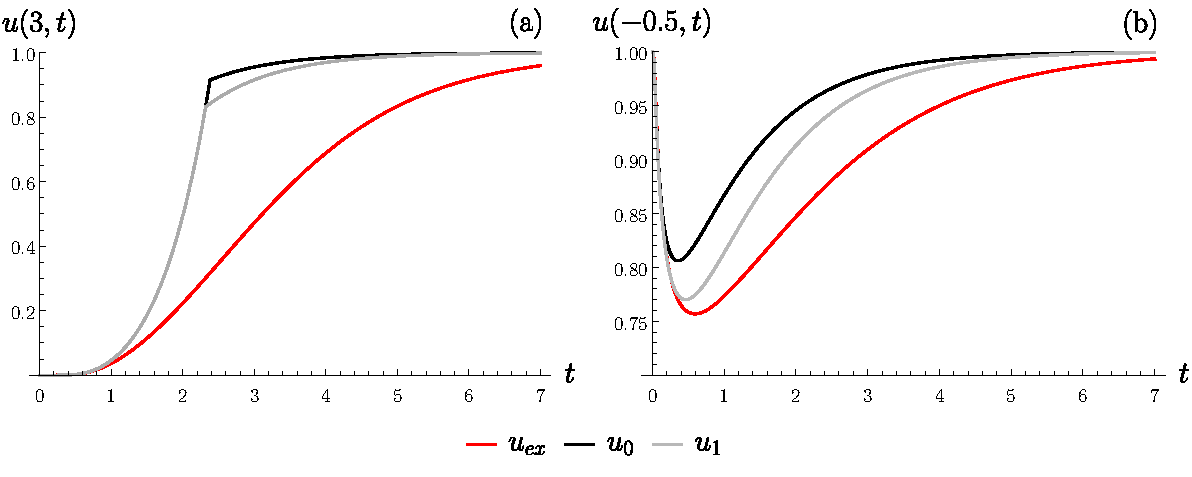
\includegraphics[width=\linewidth]{Figures/GridSimoideAlt.pdf}
    \caption{The wavefront approximants $u_0$ (full black line) and $u_1$ (full grey line) plotted in time for fixed positions $x=3$ (a) and $x=-0.5$ (b) on either side of the initial step function. For comparison the numerically exact solution $u_{ex}$ of the Fisher-KPP equation with Heaviside initial condition is shown (full red line). Panel (a) illustrates the growth and saturation of the population following the impact of the traveling front. Panel (b) illustrates the diffusion-driven depletion of a saturated population initially residing very close to an extinct population and its subsequent growth-driven recovery.}
    \label{fig:GridSimoide}
\end{figure}
\section{Refinement of the wavefront approximant} \label{sec:refinement}
Our second main goal is to provide an analytic improvement over the ``zeroth" approximant $u_0$. While we have gone beyond the conventional linear theory by matching solutions of two different linearized DEs, we have so far fully neglected nonlinearities in the DE itself. Since there exist analytic methods for taking nonlinear terms into account we set out to explore these for the purpose of obtaining a better approximation, and still in analytic form. 

To incorporate the nonlinearity, the BLUES function method comes to mind first since in \cite{Berx_2020}, this iteration procedure was already used to find approximate traveling wave solutions to the Fisher-KPP equation with a traveling-wave ansatz, reducing the PDE to an ODE. However, at that stage of development of the method, only local convergence could be attained because the saturated population boundary condition (at $x \to - \infty$) could, in general, not be satisfied. In the meantime, the BLUES function method was extended to PDEs \cite{Berx_2021} and this considerably improves its capability to deal with the problem at hand. 

Also other analytical procedures (notably ADM and VIM, briefly mentioned in Section \ref{sec:intro}) are candidates for our purpose. These methods are based on choosing a linear problem, but may differ from BLUES in the way this is done. The ADM and VIM require the linear operator to be an operator of only one coordinate, in this case the temporal coordinate $t$, to be able to set up the procedure. By making this choice, one subsequently needs to differentiate discontinuous functions such as the Dirac delta in every step of the procedure, which renders the generated approximants highly singular and hence not useful. To avoid this problem in ADM and VIM we take our piecewise-analytic approximant $u_0$ as the common starting point for ADM, VIM and BLUES, thereby putting all three methods on the same footing. 

Inspection of the methods reveals that the integrations involved in the calculation of the first-order approximants in ADM and VIM are not analytically tractable. Moreover, opting for a numerical approach in solving the integrals yields detrimental first-order corrections. These problems are much less pronounced in BLUES. Therefore, among these three candidates we opt for the BLUES function method and attempt to use it for improving upon the hitherto studied combined solution $u_0$ of the two linear PDEs \eqref{eq:linear_operator_Right_Alt} and \eqref{eq:linear_operator_Left_Alt}.

In the framework of the BLUES function method, one constructs more refined approximants to the solution of a (nonlinear) PDE in an analytic iteration procedure starting from the solution of a judiciously chosen associated linear PDE. The $n$th BLUES approximant to the solution of the nonlinear Fisher-KPP equation \eqref{eq:dimensionless_Fisher} is given by
\begin{equation}
    \label{eq:nth_order_u}
    u^{(n)}(x,t) = u^{(0)}(x,t) + (G\ast \rop u^{(n-1)})(x,t).
\end{equation} 
where the residual operator is defined as $\rop \equiv \lop - \nlop$. The details of the derivation of this result are recapitulated succinctly in the Appendix.

In principle it is possible to apply the iteration procedure to $u^{(0)}_R$ as well as to $u^{(0)}_L$. However, since $u=0$ is a repulsive ``fixed point" of the population dynamics, while $u=1$ is an attractor, the resulting approximants, in first iteration, feature long-time divergences or well-controlled long-time convergence, respectively. Therefore, and in view of the fact that $u^{(0)}_R$ is physically acceptable, we limit ourselves to improve upon $u^{(0)}_L$ and calculate $u^{(1)}_L$. Matching $u^{(1)}_L$ and $u^{(0)}_R$ then provides by definition the new moving-junction point and the new combined approximant $u_1$.  Using the ``zeroth" approximant in \eqref{eq:BLUES_First_iteration_Left} we compute the ``first" BLUES approximant for the ``left" PDE and obtain 
\begin{multline}\label{eq:BLUES_First_iteration_Left}
    u^{(1)}_L(x,t)=1-e^{-t}+\frac{e^{-2 t}}{4}-e^{-t}\text{erf}\left(\frac{x}{2 \sqrt{t}}\right)+\frac{1}{2} e^{-2 t} \text{erf}\left(\frac{x}{2 \sqrt{t}}\right)  +\frac{1}{4} e^{-2 t} \text{erf}^2\left(\frac{x}{2 \sqrt{t}}\right)\\
    +\frac{e^{-3 t}}{\pi } \int_0^1 \dd{v}
    \frac{e^{\frac{2 t }{v^2+1}-\left(\frac{x}{2 \sqrt{t}}\right)^2\left(v^2+1\right) }}{v^2+1},
\end{multline}
where the last term is a closed-form analytic expression for an integral that we fail to reduce further. The combination $u_1$ of $u^{(0)}_R$ and this new $u^{(1)}_L$ is shown in Figure \ref{fig:PiecewiseApproxAlt2} (grey lines). Note that the moving junction $x^*_1 (t)$ is now defined through $u^{(0)}_R(x^*_1,t)=u^{(1)}_L(x^*_1,t)$, which is a non-trivial transcendental equation. 

Let us examine to what extent $u_1$ provides an improvement over $u_0$. The improvement is clearly relevant for early times and is negligible for long times. This is a consequence of the fact that we keep the front $u^{(0)}_R$ unchanged. In Fig. \ref{fig:PiecewiseApproxAlt2}, panel (a),
it is conspicuous that $u_1$ is an improvement over $u_0$ in the sector for which it is calculated (to the left of the moving junction). Also the junction itself now lies closer to the numerically exact solution of the PDE. This improvement dies out as time progresses and after the relaxation time for saturation, $\tau$, $u_1$ and $u_0$ become nearly coincident, see Fig. \ref{fig:PiecewiseApproxAlt2}, panel (b). 

In Fig. \ref{fig:error}, which shows a measure of the difference between the approximant and the numerically exact solution, it is clearly seen that the first approximant $u_1$ provides a modest quantitative improvement over $u_0$, particularly (and only) for short times. The same quality of improvement is apparent in Fig. \ref{fig:Velocity} which shows the approach of the velocity to its asymptotic universal value for ``pulled" wavefronts. Qualitatively, there is no difference between $v_1$ and $v_0$. Both obey the velocity law corresponding to the ``critical case" identified in \cite{Berestycki2017}. The most important improvement which the first iteration of the BLUES method offers is visible in especially the depth and to some extent also the duration $\gamma$ of the population depletion in Fig. \ref{fig:GridSimoide}, panel (b). 

\section{Conclusions}\label{sec:conclusion}
In this paper we have presented an analytical approximant to the solution of the nonlinear Fisher-KPP equation with a step function initial condition. This approximant was found by studying the behavior of the PDE around the values corresponding to the stable ($u=1$) and unstable ($u=0$) uniform states and identifying two corresponding linear reference problems. The solutions of these linear PDEs can be joined to form a piecewise analytic approximant featuring a moving junction point. This approximant favorably meets three conditions that a proper emergent wavefront must obey: i) it must respect the boundary conditions of saturation at $x \to -\infty$ and extinction at $x \to \infty$, ii) its shape remains fixed asymptotically for large $t$, and iii) its velocity reaches a constant value ($v^* = 2$ in the case of a ``pulled" or ``critical" front) for long times. It was shown that the proposed ``zeroth" approximant $u_0$ satisfies all three requirements and the velocity asymptotics features the $1/(2t)$ leading correction of the ``critical case" rather than the $3/(2t)$ of a generic ``pulled" front. 

In spite of its simplicity, and notwithstanding the neglect of the nonlinear term in the PDE, the analytic approximant $u_0$ allows one to observe the characteristic time needed for the population to reach saturation following the impact of the wavefront, for a fixed position $x$, as well as the healing time needed to recover from a diffusion-driven depletion at positions in which the population is initially saturated but close to the extinct population ahead of the traveling wave. 

Subsequently, we have taken the nonlinearity of the PDE explicitly into account by invoking an iteration procedure, named BLUES, which pushes the Green function method beyond the linear domain. The first iteration of this approach, applied to the near-saturated domain of the population, provides an analytic approximant $u_1$ that is still presentable in compact closed form. It constitutes a (modest) quantitative improvement over $u_0$ in all of the various physical properties which we investigated and most notably in the description of the diffusion-driven depletion. Further improvement is conceivable by performing higher iterations, but at the expense of analytic simplicity of the resulting approximant. 

\appendix
\section{The BLUES function method for the Fisher-KPP equation}\label{sec:BLUES_method_pde}
Here, a setup of the BLUES iteration method for PDEs in time and one space variable is given. This section is based on the original description given in Ref. \cite{Berx_2021}. The method is applied in the context of a nonlinear PDE, given by
\begin{align}\label{eq:nonlinear_PDE}
    \nlop u(x,t)=0,
\end{align}
defined on $(x,t) \in \mathbb{R} \times [0,\infty)$ where $\mathcal{N}$ is a nonlinear differential operator. Here $u(x,t)$ represents the solution of the PDE. In the BLUES iteration procedure, one starts from a judiciously chosen related linear operator $\mathcal{L}$ and then invokes the initial condition $f(x)$ as an external source to this linear problem through the action of a Dirac-delta source in time. Accordingly, the following time and space integral, which is a two-variable convolution $u(x, t) = G \ast f \delta$, solves the rearranged inhomogeneous linear PDE, which is equivalent to the original linear PDE, 
\begin{align}
 \label{eq:rewriten_linear_operator_delta_u_appendix}
		\lop u(x, t)=\lop \int_{0^{-}}^{t} \dd{s} \int_{\mathbb{R}} \dd{y} G\left(x-y, t-s\right) f\left(y\right) \delta\left(s\right)=f(x) \delta(t)\,,
\end{align}
where $G(x,t)$ is the Green function associated to the chosen linear operator. The above description only holds if $\mathcal{L}$ contains a first (and no higher) derivative with respect to time $t$ \cite{Berx_2021}. 

The BLUES iteration method now proposes to construct a solution $u(x, t)$ to the nonlinear PDE in the form of a two-variable convolution $u(x, t) = B * \phi$, such that
\begin{align}
    \label{eq:rewriten_nonlinear_operator_delta_u}
	\nlop u(x, t)=\nlop\int_{0^{-}}^{t} \dd{s} \int_{\mathbb{R}} \dd{s} B\left(x-y, t-s\right) \phi\left(y, s\right)=f(x) \delta(t).
\end{align}
The function $B(x, t)$ is called BLUES function, and is taken to be the Green function of the relevant linear PDE. The challenge is to calculate the new associated source $\phi(x,t)$ knowing that $B \ast f \delta$ solves the linear PDE with initial condition $f(x)$ and source term $f \delta$. For this calculation one defines a time-independent residual operator $\rop \equiv \lop - \nlop$ and makes use of the implicit identity
\begin{equation}
    \label{eq:phi_identity}
    \nlop (B\ast\phi) = \phi(x,t) - \rop (B\ast\phi) = f(x)\delta(t), 
\end{equation}
which follows directly from the Green function property of $B$ with respect to the chosen linear PDE.

To obtain the solution to the nonlinear PDE with initial condition $f(x)$, equation \eqref{eq:phi_identity} can be rewritten 
\begin{equation}
    \label{eq:phi_identity_re}
  \phi(x,t)  = f(x)\delta(t) +  \rop (B\ast\phi), 
\end{equation}
and iterated in order to calculate an approximation in the form of a sequence in powers of the residual $\rop$. The zeroth iteration is 
\begin{equation}
    \label{eq:zeroth_order}
    \phi^{(0)}(x,t) = f(x) \delta (t),
\end{equation}
such that the $n$th iteration with $n\geq1$ becomes
\begin{equation}
    \label{eq:nth_order}
    \phi^{(n)}(x,t) = f(x) \delta (t) + \rop (B \ast \phi^{(n-1)}).
\end{equation}
Consequently, the $n$th analytical approximant to the solution of the nonlinear PDE is found through the two-variable convolution
\begin{equation}
    \label{eq:nth_order_u_appendix}
    u^{(n)}(x,t) = B \ast \phi^{(n)} = u^{(0)}(x,t) + (B\ast \rop u^{(n-1)})(x,t).
\end{equation}

\bibliography{BLUES.bib}
\end{document}